\section{Experiments}
We choose two state-of-the-art models BERT \cite{devlin2018bert} and ERNIE \cite{sun2019ernie} as our baselines. 

BERT is absolutely a milestone in NLP domain. Lots of NLP tasks achieve great improvements with BERT due to its pre-trained knowledge on natural language, including syntax and semantic features. 
Following the idea of pretrained language model, some other works come up to further improve the performance of BERT, such as ERNIE, XLNet \cite{yang2019xlnet}. 
Since pretraining on a large corpus is quite time-consuming, we finally choose \textbf{\textit{BERT-Base for Chinese}}\footnote{https://github.com/google-research/bert}  and \textbf{\textit{ERNIE 1.0 Base for Chinese}}\footnote{https://github.com/PaddlePaddle/ERNIE} as our baselines as they are the only two publicly released models pretrained on the Chinese corpus, where BERT trained on Chinese wikipedia and ERNIE trained on Chinese Wikepedia, Baidu Baike, Baidu news and Baidu Tieba. 
% trained dataset these two models use

On the basis of BERT, ERNIE further modeled entity and word information to integrate knowledge to some extent.
As these two models are pretrained using large corpus, we %first 
suppose that they have implicitly learned commonsense.\JQ{commonsense, finetune分分合合}

For our task, we calculate perplexity of each phrase $\{w_1, w_2, ..., w_m\}$ using the pretrained language model by applying the following formula:
\begin{equation}
\begin{split}
&perplexity(phrase) = p(w_1, w_2, ..., w_m)^{-1/m} \\
&\approx \sqrt[m]{\prod_{i=1}^{m}\frac{1}{p(w_i|w_1,...,w_{i-1},w_{i+1},..., w_m)}}
\end{split}
\end{equation}
and we choose the one with higher score as the commonsense contradiction phrase.



\subsection{Fine-tune using E-commerce data}
Our dataset are collected from user query on an E-commerce platform. Although the data cover numerous scenarios in daily life, the word distribution is different from Chinese Wikipedia that used in the pretraining process of BERT and ERNIE. Therefore, we use the E-commerce data to finetune the model. The details of data used are shown in the Table \ref{tab:DetailData}.

As the training process are quite slow due to the large data size, we only conduct the fine tune process on BERT.% model.

\begin{table}
	\small
	\centering
	\begin{tabular}{cc}
		\toprule[1.1pt]
		Data source & Data Size \\
		\hline
		XiaoHongShu & 15 millions \\
		Baidu Baike & 10 millions \\
		Tao GongLue & 6+ millions \\
		E-commerce descriptions & 3+ millions \\
		\bottomrule[1.1pt]
	\end{tabular}
	\caption{Details of E-commerce data used for fine tune}
	\label{tab:DetailData}
\end{table}

\subsection{Fine-tune using CoCo dataset}
As we know that, human acquire common sense from his experience or inference based on his knowledge, instead of being told that something is absolutely right. Our released benchmark is also designed to measure if a machine has the commonsense judgment. Hence, we argue that commonsense of machine should be learned implicitly from large corpus or inferred by knowledge acquired from external knowledge base, instead of tuning on a specific similar training set.
%in ConceptNet or Probase. 
%It should be noticed that the commonsense concerned more about the intrinsic property of things instead of some facts.  

However, we are also curious about how much the pretrained language model like BERT can learn from short text. Therefore, we split our dataset into train/dev/test set and use train set to finetune the basic BERT and ERNIE.

To avoid the statistical clues revealed by word, we count frequency of each word appeared in either positive or negative side for each sample. Those words that have obvious statistical feature will not appear in the train set and test set simultaneously.

Finally, the data size of our train/dev/test set are 8343/454/432. The results of finetuned BERT/ERNIE using all CoCo training data are shown in Table \ref{tab:ExpRes}. Besides, the learning curves with varying amounts of  training data will be presented and discussed in the last part of this section.  

For both BERT and ERNIE, we fine tune the network by adding a fully-connected layer over the first token obtained by the last layer in the original model, which is shown in Figure \ref{fig:tuneNet}. Because our task needs to compare two phrases in a data sample, hinge loss is used to do the optimization. Both initial learning rate are set to be $2e-5$, and training epoch is 3. Other parameters are the same as the default settings given by the official tutorial.

\begin{figure}[h!]
	\centering
	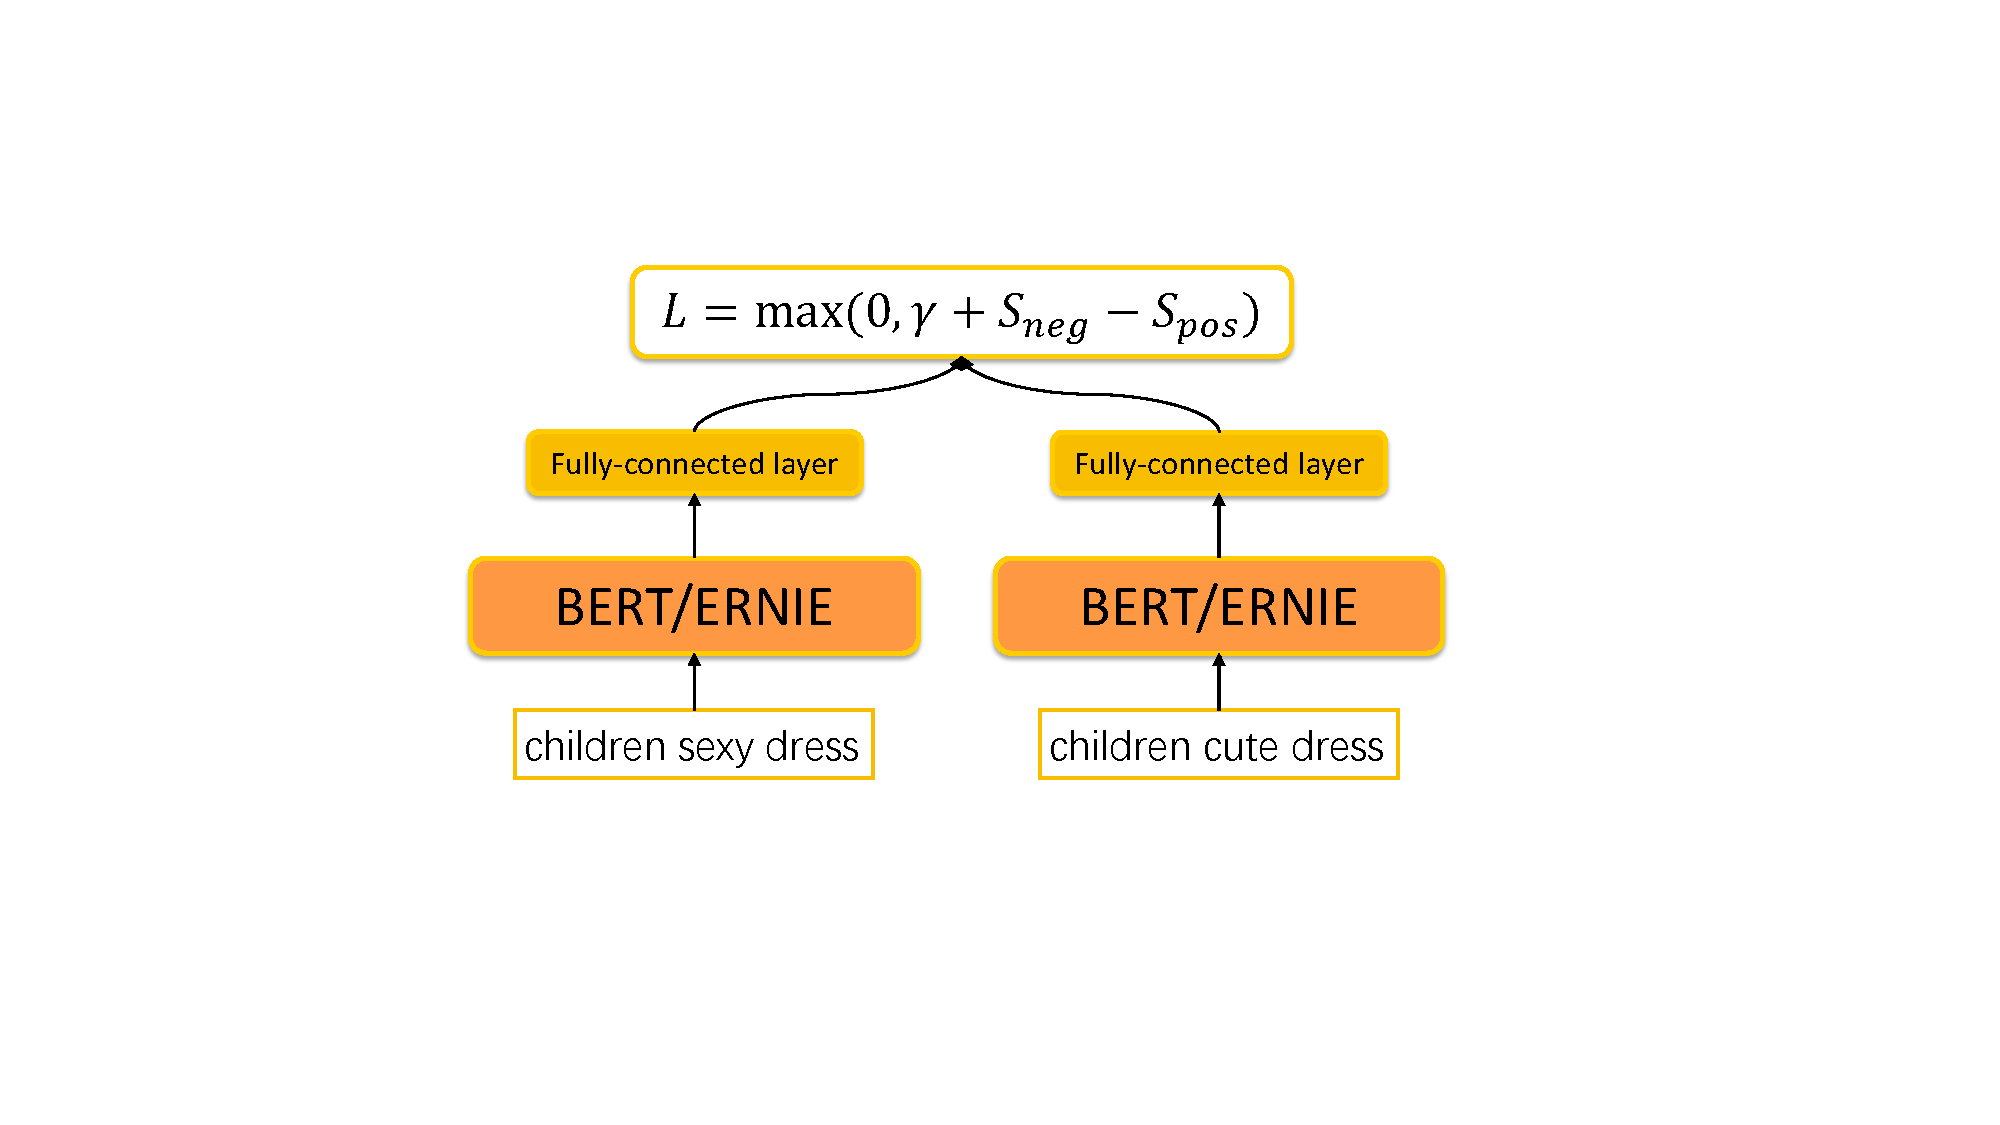
\includegraphics[width=0.8\columnwidth]{images/fineTuneNetwork.pdf}
	\caption{Model of Fine-tuned BERT\&ERNIE}
	\label{fig:tuneNet}
\end{figure}
%\KZ{translate the chinese in the figure to English.}
%\subsection{Experimental Setup}


\subsection{Human Evaluation}
We also conducted human evaluation on our dataset. 100 samples are randomly selected from dataset and distributed to two people, who did not participate in the construction or quality verification process of the dataset. The average of their accuracy are considered as the human performance borderline. 
%Results of experiments are shown in Table \ref{tab:ExpRes}.




\subsection{Results \& Analysis}
Results of all models are shown in Table \ref{tab:ExpRes}. As this is a binary classification problem, the random baseline leads to 50\% accuracy rate. 
The best baseline evaluated on CoCo dataset achieves accuracy of 0.6447. When fine-tuned on CoCo train set is permitted, the best baseline can achieve accuracy of 0.7662 on CoCo test data. However, these two results are both far below the human performance (0.95), demonstrating that our released benchmark is much easier for human, but still remains a great challenge for current state-of-the-art machine. Notice that all results surpass the random choose (0.5), showing that the pretrained model %can indeed 
try to memorize numerous amounts of information.

\begin{table}
	\small
	\centering
	\begin{tabular}{p{2.5cm}p{2cm}p{2cm}}
		\toprule[1.1pt]
		Models & Accuracy (CoCo) & Accuracy (CoCo testset) \\
		%Models & Accuracy on CoCo & Accuracy on CoCo testset\\
		\midrule[0.75pt]
		Random & 0.5 & 0.5\\
		%\hline
		BERT & 0.5992 & 0.6019\\
		Fine-tuned BERT (E-commerce)  & \textbf{0.6447} & 0.6667\\
		Fine-tuned BERT (CoCo) & - & 0.7471\\ %0.7719\\
		ERNIE & 0.6007 & 0.6944\\
		Fine-tuned ERNIE (CoCo) & - & \textbf{0.7662} \\ %0.7847\\
		\midrule[0.75pt]
		Human&0.95&0.95\\
		\bottomrule[1.1pt]
	\end{tabular}
	\caption{Accuracy of models on CoCo dataset}
	\label{tab:ExpRes}
\end{table}


Without seeing any related data in CoCo train set and evaluated on the whole CoCo dataset, the basis pretrained language model BERT (0.5992) and ERNIE (0.6447) perform nearly the same. 
The gap between these two models is considered due to the different size of pretraining data. As BERT uses only Chinese Wikipedia data, and ERNIE uses %another 
additional three data sources (include Baidu Baike, Baidu news, Baidu Tieba)  Except for Chinese Wikipedia, ERNIE may store more relation statistics between words. We also find that the accuracy of BERT improves after fine-tuning using E-commerce data, indicating that the dataset with more similar domain knowledge could further improve models' performance.

 Despite of this small improvement, the performance of fine-tuned BERT using E-commerce data is still far from human. We argue that current design of pre-trained language model like BERT or ERNIE can not exactly learn commonsense knowledge from large amounts of training data, it needs to integrate external knowledge in some ways to be further %evaluated 
improved on our released benchmark. Besides, our dataset aimed at short text which also makes it more difficult for machine to understand directly as it is absent of enough context and standard syntactic structure.

%the fine-tuned BERT by E-commerce data achieves 

Take the split CoCo data into training process, both BERT and ERNIE get further improvement. The influence of varying amounts of training examples is shown in the next part. %sub-section.   


%\subsection{Baseline Analysis}

\subsection{Learning Curves}
%\label{hi}

%To better understand the learning performance of both BERT and ERNIE, we fine-tune these two models on different size of CoCo training data.

To extrapolate how current two models BERT and ERNIE perform with various amount of data, we fine-tune these two models by varying CoCo train set. However, we remain the num of training epochs and initial learning rate unchanged. The other hyper-parameters are also kept the same. To deal with learning stabilities, each data point is the average of 4 runs. The resulting learning curves are plotted in Figure \ref{fig:learnCurve}. 

We observe that the pretrained ERNIE performs much better than BERT when the training samples are few, but their performance are getting close with increasing training data. 
The possible reason is that ERNIE try to mask the entity and the whole word during its language model pretraining process, which may help ERNIE to better learn the relation between words. However the BERT only regard each Chinese character as a mask unit during pretraining. 

%The possible reason is that ERNIE use more training data during pretrained process, may memorize more relation statistics between words. %However, ERNIE still defeats BERT little  

After using nearly 90\% of total dataset, these two models can merely achieve around 0.75, which is still substantially lower than human performance.
% We hypothesize that they will plateau quickly. (no instance)

%However, we hypothesize that both models need very large associated training data to 

\begin{figure}[h!]
	\centering
	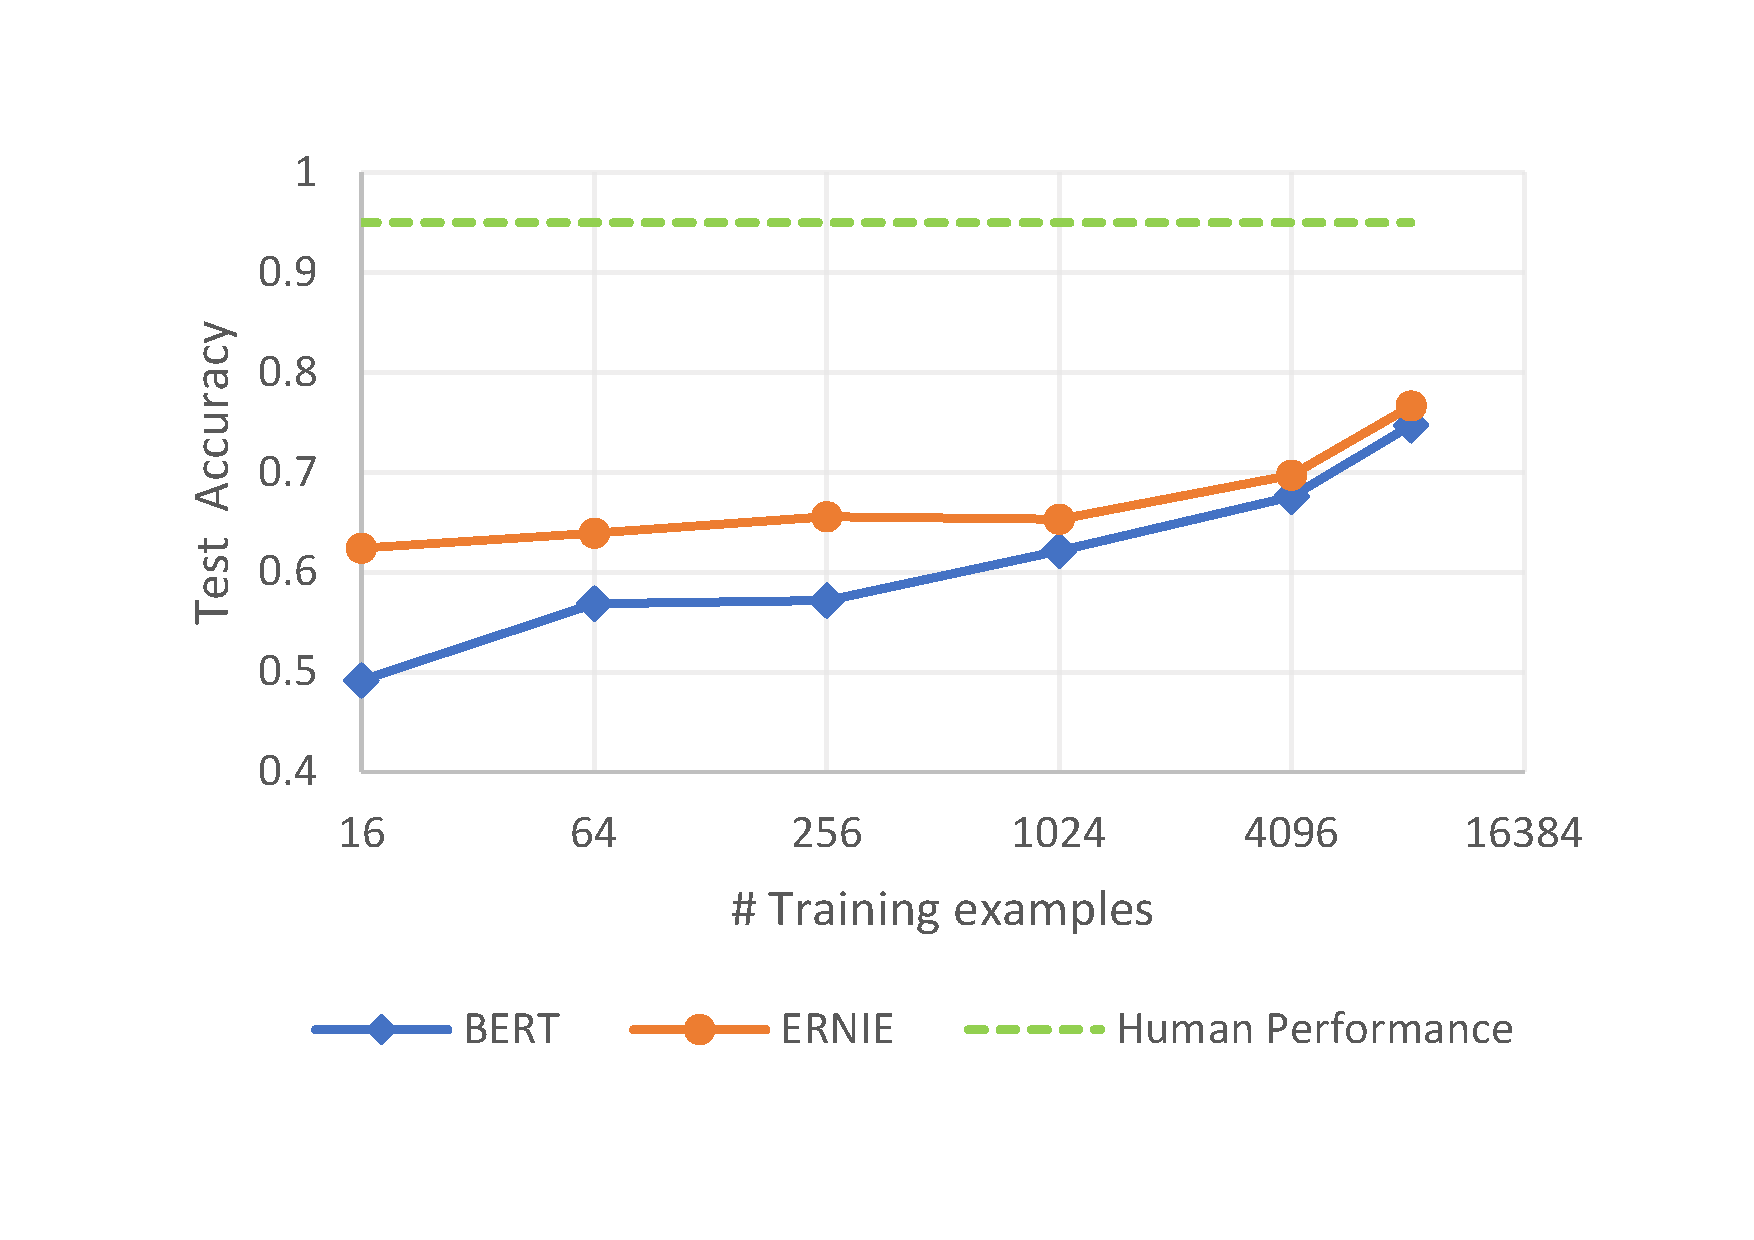
\includegraphics[width=0.9\columnwidth]{images/learnCurveLine.pdf}
	\caption{Accuracy on CoCo test set for BERT/ERNIE fine-tuned with varying amounts of data}
	\label{fig:learnCurve}
\end{figure}

